% This file is iccc.tex.  It contains the formatting instructions for and acts as a template for submissions to ICCC.  It borrows liberally from the AAAI and IJCAI formats and instructions.  It uses the files iccc.sty, iccc.bst and iccc.bib, the first two of which also borrow liberally from the same sources.


\documentclass[letterpaper]{article}
\usepackage{iccc}
\usepackage{times}
\usepackage{helvet}
\usepackage{courier}
\usepackage{hyperref}
\usepackage{graphicx}
\usepackage{caption}
\usepackage{subcaption}
\usepackage{comment}


\title{Steganography: Maximizing Waveform Digital Audio Capacity\\
Paper type: Measurement Paper }
\author{James Bach, Jonathan Smith\\
Computer Science Department\\
Florida State University\\
Tallahassee, FL 32306  US\\
bach@cs.fsu.edu, jonathan3.smith@famu.edu\\
}
\begin{document} 
\maketitle

\section{Abstract}
Steganography is often described as the "art and science of information hiding." This art and science is based around three major design considerations: security, robustness, and capacity. Capacity is the most important design consideration because without a sufficient quantity, the ability to store the payload and any additional data to make it secure and robust is not possible. Transitively, when considering the application of technical steganography, if an attacker is aware that a file contains a secret message, the robustness and security of the message is the final bastion for the secret to persevere. Therefore, having the capacity to support these designs makes it the fundamental concept. This research focuses entirely on determining the maximum capacity of an uncompressed digital audio file with a minor application of security to prove its validity. The method of determining this capacity in the underlying file format involves an n-bit replacement method, an extension of the least significant bit method. The upper bound capacity measurement is validated by the lack of human detection and because of our security mechanisms, it also evades many computer based detection methods. Our focus is the Microsoft Windows standard uncompressed digital audio waveform sound file (WAV). This Waveform audio file format was created by IBM and Microsoft Corporation in 1991 and introduced with the release of Windows 3.1 as the standard to store an analog audio bit stream.     


\section{I. Introduction}

Cybersecurity is a growing discussion in business, education, politics, and technology. Threats are emerging that cause concern for the safety and security of the global community. In the dangerous world of espionage and other types of security-sensitive missions that would require cyber-communication, situations arise where an initiator needs to send a secret message to a trusted entity that may cross enemy territory. The enemy territory in this case could involve networks that are not secure, behind enemy lines. Adversaries effective at monitoring transmissions will likely be eavesdropping all messages. The messages could pass through public access points where non-adversaries may also be exposed to these messages. The practice of using steganography makes secret communication harder to detect because the secret is hidden in plain sight. 

On the other hand, the same adversaries of rogue government agencies, black hat hackers, malicious agents, and others performing illegal activities such as child pornography, arms dealers, drug dealers, and human trafficking, use steganography to hide their business transactions, plans, and data. In many cases, detecting their messages and recovering their secrets could be paramount to saving the lives of potentially millions of innocent people. 

There are two particular types of steganography: linguistic and technical. The linguistic steganography methods include encoding messages based on using details and characteristics of the actual message. Technical steganography exploits how the message is stored on mediums and in many ways manipulating their underlying file format.\cite{survey} Some examples of common mediums used are image, audio, and video files.

The details of file format design is something overlooked because our applications for development transparently handle files and many of them are universal. Many file formats have been around for twenty to thirty years and using them in applications and development has been simplified and generalized with high level libraries and utilities. We sometimes forget that the files contain meta data which can reveal everything about a file. Users may not realize how much reserved space versus actual data is used in a file format. Many of the applications that use the meta data extract what they need to seamlessly provide the user interface with the proper information.  

Although most steganography has relatively little openly available research, image steganography might be the most saturated. Digital audio steganography has far less applied research.  \cite{avcibas2006audio} There are no visible research discussions that explore the upper bound capacity a file could potentially store, but rather just details about the methods of digital audio steganography. These methods do not necessarily utilize the full capability of the file but iterate among other previously used methods or improve security with clever ways to encode the data. These works focus on the security of the message rather than how large the payload can be. This research applies the concept of exploiting the digital audio file format structure to hide a payload. The focus is determining the upper bound capacity available in the waveform digital audio file which is a standard uncompressed digital audio file used widely in Windows, Linux, and Mac OSX, the common modern operating systems used today.

In the following sections are works that have inspired and strengthen this research, an explanation of steganography to provide a perspective of the decisions made in this research, a brief introduction to digital audio and human hearing to connect conclusions made from this research, and several sections on the methods, analysis, and results of the experiments of determining the maximum effective steganographic capacity of a waveform digital audio file. 

\section{II. Related Works}
There is a plethora of research in steganography in image files and graphics, however, digital audio steganography and audio steganalysis is a relatively unexplored domain. The success of achieving secret communications, is determined by the inability to distinguish a difference between the "stego-signals" and "cover-signals." \cite{avcibas2006audio}
	
The most relevant works related to this research is from the standpoint of raising the bit index value from the LSB value to a higher value to improve capacity and robustness for their steganographic model with respect to file alterations. Similarly, they validate their results with spectrograms and spectral distortions. \cite{gopalan2015imperceptible} This paper discusses a model similar to our research but does not elaborate on the theoretical maximums just that there is potential effective capacity available. Another such work discusses general methods of increasing capacity primarily by the use of direct embedding into audio files using the n least significant bits.\cite{cvejic2002increasing} They mention the use of the human auditory system and the analysis of the spectrograms, when making their claims.

Another work performs a similar function of using AES encryption of the payload with the digital audio steganographic method of spectrum spread to optimize the ability to conceal and protect their secret. \cite{khan2011optimized}  In our research, we develop a payload of an encrypted file system that is embedded using a modified least significant bit, using n-bits. Spread spectrum is discussed in later sections along with the approach taken in this research.

The work "Adaptive Lossless Digital Audio Steganography" uses two techniques based on integer transform focusing on the frequency domain and the spacial domain. The spacial domain approach has the embedded data spread over a long period of time. The frequency domain approach modifies the signal segments based on human auditory system temporal characteristics. The human auditory system research shows that the natural, slight distortion at high volume sound makes the modifications inaudible. \cite{1599886} Our research analyzes the implications of modifying bits as a spatial domain determining the maximum capacity that can be used and this work validates the effectiveness of our research's experiments and its relationship with the human auditory system mentioned in a later section. 

There is a steganographic application called DeepSound which can be found at \href{http://jpinsoft.net/DeepSound/Overview.aspx}{http://jpinsoft.net/DeepSound/Overview.aspx}
that performs a similar function to StegoMax. This will embed files into FLAC, WMA, WAV, and APE. This also offers the feature of 256-bit AES encryption of the payload. Our research replicates many factors of this particular application. In their documentation they just briefly discuss using 50\%, 25\%, and 12.5\% of the audio file, considering them as low, normal, and high quality respectively. There are a several other application but this one is the most significant.


\section{III. Steganography}
Introducing the specifics of steganography, the history begins in ancient Greek means "Covered Writing." Some of the first ever known steganographic practices involved a Greek general tattooing messages on a slaves shaved head. The general would send the slave to the destination after his hair grew back. The receiving commander could then shave the slave's head and receive the message. Should the slave become captured, the captors would be none the wiser.\cite{survey} Information hiding methods have come a long way since ancient Greece and have a diverse spectrum of utility and application. 

Discussion around information hiding typically involves three design concepts: security, capacity, and robustness. These three ideas encompass all the major criteria required for effective practice when evaluating steganography and watermarking.

\subsection{Security}
There should be no doubt that providing security for a secret message or a payload is an important design decision when applying steganography. The design of security also covers the concealment factor involved, making the payload harder to detect, yet both are necessary to be effective. When the presence of a payload is detected by an adversary, the only thing preventing them from discovering what the secret is will be based solely on any security mechanisms in place. 

For example, let a secret be a plain text message (also referred to as a null cipher) in the least significant bits and the adversary is eavesdropping to intercept all messages. Assuming the adversary successfully intercepts the message, they could apply a least significant bit extraction and recover the plain text secret. The goal of security is to make this process more difficult and hopefully impossible for the adversary to gain the secret. In the proverbial bag of tricks there are several easy, yet effective, mechanisms that can be applied to strengthen the security of the message.

Furthering the previous example, a simple security mechanism that can be applied to a null cipher would be to make the real secret message be a combination of every second letter of every word. This is an exact example used in World War II. A null cipher actually sent by a German spy:
\begin{quote}
"Apparently neutral's protest is thoroughly discounted and ignored. Isman hard hit. Blockade issue affects pretext for embargo on by-products, ejecting suets and vegetable oils."
\end{quote}
The real secret in this message is: "Pershing sails from New York June 1." This refers the military movement of the United States Army General John. J. Pershing.
\cite{johnson1998exploring} 

Another trick in the bag and the primary security mechanism applied in this research is AES encryption. Encryption typically is challenging to introduce in steganography due to the extremely small sizes of the mediums. This introduces a minimum requirement for our goals but does not limit the applicability of the capacity research.

An aspect of security in steganography worth mentioning involves the endpoints of the message. There is often a software platform that performs the embedding and extracting, much like the application of this research. In methods using special patterns when embedding a payload as the primary means of security are used, should the platform for embedding and extracting become compromised, the whole system will fall. If an attacker recognizes that the ability to find this message in the image is far more expensive to discover rather than take the platform itself, the attacker will target the endpoints and the steganographic methods are trivial.  

\subsection{Capacity}
In any given file, there is only so much storage that can be exploited before the ability to detect a message becomes noticeable because the original file is noticeably altered or even corrupted. In designing around capacity, there is strong consideration of what size payload can be used along with what mechanisms are used to make it more robust, and additionally what security methods are applied to the payload. The overall effectiveness of the steganography depend on these three factors.  

A platform could be designed by using a LSB method and with a simple security mechanism in place could be to use every other LSB. This would reduce the capacity by 50\% but could better scramble the message. However, this does not always mean great security but does however reduce the capacity potential. In Figure \ref{fig:steganal} from later sections shows the LSB being taken from the first half of the message.

In making the payload more resilient, the message could have mechanisms in place to recover altered data. The recovery process is often a mathematical relationship such as a parity or hamming distance. Introducing mechanisms like this will greatly increase the capacity requirement. 

It should now be apparent that capacity plays the most important role of the three seeing as how many mechanisms that improve robustness and security require more storage space. Capacity in digital audio steganography in other methods mentioned in a later section is relatively small. The techniques used to store the payloads involve non-maximal methods. Although some of them provide for more capacity than others, the final form of every digital audio file is a binary file. This research is solely based on maximizing the data stored in the final binary form of the previously mentioned waveform digital audio file.


\subsection{Robustness}
A message may not be detected by an eavesdropping adversary or unknowing user, however it can most definitely be destroyed. The destruction can be both intentional and unintentional through modification of the file. An eavesdropper could take the message and alter a few bits or bytes, rendering the entire message usefulness to the destination. A common scenario where the design focuses on robustness is watermarking for Digital Rights Management (DRM). Robustness is important to watermarking in order to remain effective against unwanted distribution or tampering. Watermarking is discussed briefly in the next section.

In networking, a particular method in the data-link layer of the OSI model uses Hamming codes for error detection and correction. Code words and Hamming distances are can be used for improving robustness of a secret when used for steganography. This greatly increases the capacity requirement, should the whole message be made to be more robust. In particular, distance codes would be of size 2d+1 where d is the number of errors to correct.\cite{tanenbaum2003computer} 

\begin{figure}[h]
    \centering
    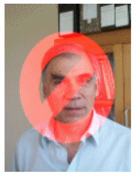
\includegraphics[width=3cm]{images/watermark.png}
    \caption{This shows a watermark present in the image, this watermark would destroy the image if it were removed. The image is created by overlaying the watermark onto the original image.}
    \label{fig:ukstego}
\end{figure}

\subsection{Watermarking}
Watermarking is a subset of information hiding that focuses more on the medium it is associated with. In opposition to steganography where secret communication is the main objective, watermarking attempts to preserve copyright or integrity. Due to this particular objective, it is incredibly important to have robust mechanisms in place. Most watermarking does not intend to be concealed but rather seen to make others aware of some ownership rights or illicit activities should the file not be where expected. Often watermarking can be designed to self-destroy the file if the watermarking has been removed or copied. In Figure \ref{fig:ukstego}, the image has a watermark that if removed, would destroy the image or impede successful copying of the file. \cite{ukstego}



\section{IV. Digital Audio}
In the time before computers and other advanced audio technologies came into the picture, analog audio techniques were performed for recording sound and playing sound. Analog audio is sound that has been stored in the form of a continuous signal on to some media such as magnetic tapes or records. The techniques often involved recording air pressure with a transducer, effectively recording sound waves by converting sound energy to electrical energy to a medium. Eventually, computers became more advanced and the ability to record sound with far more precision and quality lead to the development of digital audio. 
 
\begin{figure}[h]
    \centering
    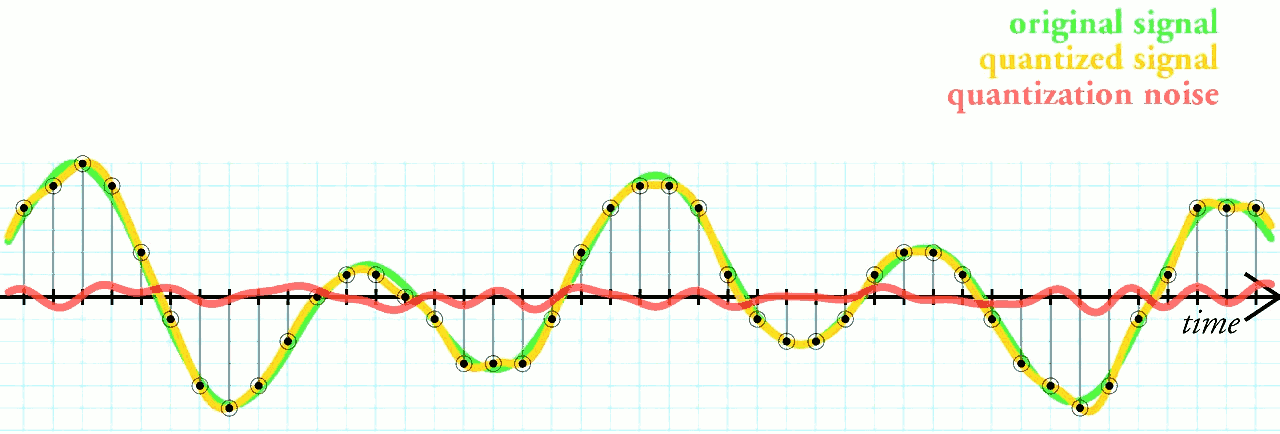
\includegraphics[width=8cm]{images/quanterrr.png}
    \caption{The audio wave is sampled uniformly from the original signal. The extrapolation between the sampled points leads to an error from rounding and truncation shown by the quantization noise line.}
    \label{fig:quanterr}
\end{figure}

Digital audio allows audio signals to be encoded in a digital format. A particular method used in this research of achieving this digital format is the use of pulse-code modulation (PCM). Pulse-code modulation  uniformly samples the analog signal to record audio. Next, the samples are quantized to fit a digital range. Quantization is a concept of mathematics and digital signal processing used to map larger sets of data into smaller sets by techniques such as truncation and rounding. This introduces an error which is considered quantization noise. In Figure \ref{fig:quanterr}, an audio wave is shown with each dot representing uniform samples. The quantized signal extrapolated from the samples have a rate of error from rounding and truncation, shown by the quantization noise line. \cite{quantpic}  


\section{V. Methods of Digital Audio Steganography}
In digital audio steganography, there are only a few methods generally mentioned for hiding a payload within a cover-signal. This may be due to the limited research in the field, the lack of applicability to standard use, the desire to keep such knowledge private and secret, and that there is only so much that can be done with a file with regards to hiding data. 
\begin{itemize}

\item \textbf{Low-bit Encoding}\\
In almost all steganography, whether using images, audio, or video, there is a method of low-bit encoding. Encoding the least significant bit typically alters the host file in such a way that goes unnoticed such as a fraction of a percent difference in color and indistinguishable audio or video signal changes. This applies across almost all file types regardless of compression. 

In the case of this research, the waveform files are uncompressed and there is a significant range of bits that can be altered and still be indistinguishable from the unaltered host file. The approach we take is most closely related to this particular method except its more of an n-LSB method. 



\item \textbf{Echo Hiding}\\
This method introduces an echo to the audio file where the secret is embedded which can be seen in Figure \ref{fig:echo}.\cite{kaur2015data} 
The echo has to modify amplitude, decay rate, and delay time of the original analog audio signal to be effective.  \cite{meghanathan2010steganalysis}

\begin{figure}[h]
    \centering
    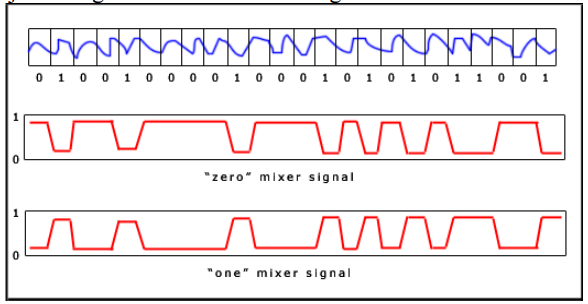
\includegraphics[width=8cm]{images/echo.png}
    \caption{"In echo hiding, information is embedded in the audio cover file by introducing an echo into the discrete signal. One echo
signal produced in the original signal embeds only one bit of information. Therefore in this original signal is split into
blocks and echo’s are inserted and these echo’s then embed the information bits in them. When the encoding process is
completed the blocks are then joined together to form the final signal."}
    \label{fig:echo}
    
\end{figure}


\item \textbf{Phase Coding}\\
The phase encoding method breaks up the original audio signal into a number of smaller segments equal to the length of the message. Then the message is encoded by performing phase shifts in each segment relative to being a binary 0 or 1. This method is significantly strong against detection but particularly low capacity capabilities. 

\item \textbf{Spread Spectrum Coding}\\
This method will attempt to sporadically hide bits throughout the signal randomly, however this often introduces a noise that can detected. The noise that occurs comes from the fact that the message is spread across the entire audio spectrum.   

\end{itemize}





\section{VI. StegoMax}
StegoMax is the steganographic platform developed for this research which performs embedding and extraction into Microsoft 16-bit PCM WAV files using the calculated maximum capacity as the storage location within the file. The process of developing this system required a deep understanding of the WAV file format and RIFF concept. In the following sections, the file format will be briefly discussed to provide a basic understanding, the assumptions for the system will be enumerated, and experimental methods and considerations will be identified. Figure \ref{fig:diagram} shows the data flow of the system.

\begin{figure}[h]
    \centering
    \includegraphics[width=10cm]{images/diagram.png}
    \caption{The StegoMax system allows the user to create an encrypted FAT file system volume, which can be used to store a secret message. Then that file system is embedded into the cover signal, creating a stego file.}
    \label{fig:diagram}
 
\end{figure}

\subsection{File Format}
The waveform audio file format (WAV) standard is a subtype of the resource interchange file format (RIFF) standard. RIFF is a tagged file structure format specifically designed for multimedia resource files. The tagged chunks provide a modular approach that has a primary advantage of being extensible and future-proof.\cite{riffspec} Additionally, the WAV file chunk metadata fields have specifications for their endianness making the system portable among Windows, Linux, and MacOSX. Another example of a RIFF subtype is an Audio Video Interleaved (AVI) file which contains audio and video commonly used for PC video.  

\begin{figure*}[ht]
    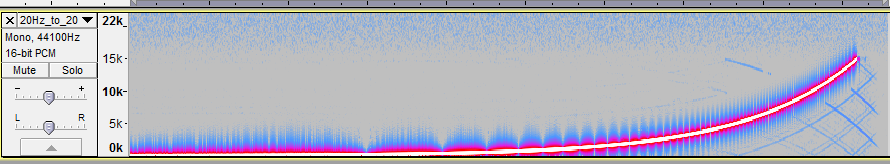
\includegraphics[width=18cm]{images/humannoise.png}
    \caption{Spectrogram of a mono channel simple sound from 20Hz to 20kHz, the approximate range of human hearing.
 }
    \label{fig:noise}
\end{figure*}


The layout and size of the meta data fields for each chunk of WAV files can be seen in a later Figure \ref{fig:heatmap}. The chunk and subchunk ID fields contain big-endian magic numbers 0x52494646, 0x666d7420m, and 0x64617461 corresponding to 'RIFF', 'fmt', and 'data', respectively.  

The data chunk layout is determined by the formatting chunks such as the number of channels and the bits per sample. Mentioned previously, the specific WAV file analyzed in this research is '(Microsoft) signed 16-bit PCM', making bits per sample field be 16. The PCM, or pulse code modulation, method also previously mentioned is used for encoding audio into a digital format. 



\subsection{Assumptions} 
The StegoMax research is designed with several assumptions in mind. The assumptions will further specify why certain decisions were made and to elaborate on certain considerations. 

\begin{itemize}

\item \textbf{Adversary}\\
This research relies on the assumption of having a passive adversary rather than an active adversary. Active adversaries would be countered with watermarking and fingerprinting, making the information hiding more robust and harder to destroy. The passive adversary entails a listening party that could bring damage or harm should they detect and discover the secret present in the message. The Simmons' "Prisoners Problem" \cite{simmons1984prisoners}, summarized below, describes the role of a passive adversary: \begin{quotation} 
"Alice and Bob are in jail and wish to devise an escape plan. All their communication
is observed by the adversary (the warden), who will thwart their plan by transferring
them to a high-security prison as soon as he detects any sign of a hidden message. Alice and Bob
succeed if Alice can send information to Bob such that the warden does not become suspicious."\\ - \cite{cachin1998information}

Another important aspect to mention is that the adversary will not have both embedded secret copy and original copy of the file. There are numerous ways to determine file differences one of which is a simple checksum, which would easily reveal the file alteration. If this does happen to occur, detection is imminent and the security of the message is all that remains to keep the adversary from knowing the secret. 
\end{quotation}



\item \textbf{Human Hearing}\\
The human ear has the ability to encode sound waves into electrical impulses which are sent to the brain to process what we perceive as sound. The technicalities of how ears process sound will not be addressed in this paper. However, it should be noted that the capability of human hearing has a range of frequency of approximately 20Hz to 20kHz, where 1kHz to 4kHz is the most sensitive. \cite{digitalprocess} This is why the bit modifications made to support the secret messages are not noticeable to a passive adversary. 

A spectrogram is often used to show a spectrum of frequencies, especially in audio analysis. Figure {\ref{fig:noise}} shows a spectrogram of a simple noise being made from 20Hz to 20kHz, the approximate range of possible human hearing. The darker colors represent the stronger sounds and the light or faded colors and noise pattern represent faint, insignificant, or inaudible noise. This is particularly relevant given that in the much later Figure \ref{fig:spectrogram}, although the modified file differs from the original file, the sound is insignificant and/or inaudible. 

In the first 0.05 seconds of the particular clip from the previously mentioned figure, the original has artificially empty data such as forced or truncated zero quantization, seen on the top spectrogram. The spectrogram below has the lower four bits modified and now an inaudible noise pattern is present.    


\item \textbf{Entropy}\\
In information theory, entropy is the measurement of randomness or in other words, the "uncertainty in a series of numbers or bytes."\cite{clausius1976application} A World War II cryptographer, Claude Shannon, originally defined entropy and provided an evaluation for measuring it in a message. Shannon's calculation would measure something like pure white noise at the theoretical max.\cite{shannon2001mathematical} The bounds of Shannon's formula are [0,8] and measured as follows:

$$ H = -\sum_{i=1}^{n} p_i \log_2 p_i$$

High entropy in steganography is fundamental in improving defense against steganalysis. If alterations of a file are made for a secret message, the modifications could reduce the entropy within the file such as in Figure \ref{fig:steganal}. This research applies a high entropy model using an encrypted file system to reduce the threat of detection. The assumption made here provides that the encrypted file system has high Shannon entropy. \cite{dodis2005entropic}
 
\begin{figure}[t]
    \centering
    
\includegraphics[width=5cm]{images/lena_lsb.png}
    \caption{An application of steganalysis showing an extraction of the least significant bit of an image file. The entropy of bits is drastically different between the top half and bottom half. Steganalysis has undoubtedly shown steganography present in this file. 
 }
    \label{fig:steganal}
\end{figure}

\item \textbf{Compression}\\
Data compression involves reducing the capacity requirement of the secret by encoding the data to use less bits. There are two reasons compression is not considered in this research, the compression could have an adverse effect on entropy and compression of an encrypted file of high entropy is often ineffective.  \cite{shannon2001mathematical}

The one aspect of compression worth mentioning is that files placed in the file system could be compressed to provide additional storage within the file system itself. This nested compression could effectively increase the carrying capacity but does not increase the capacity stolen from the file. This particular application is only relevant to our AES encryption model and not the maximum payload within the file does not change.

\item \textbf{INFO and TAG/ID3 chunk}\\
The RIFF format supports an extended meta data chunk ID containing a magic number translating to "INFO". The presence of this chunk allows for additional categorical data such as artist, track, or album. 

Another chunk occasionally appended to audio files is ID3 meta data. This chunk is defined by the magic number at the beginning of the chunk, 0x5441470d0a or 0x4944330d0a translating to "TAG" and "ID3", respectively. \cite{nilsson2004id3v2} ID3 is a standard for describing audio information such as title, artist, or genre. The standard was developed from the 1990's and has been updated a few times since.  

The existence of these chunks are optional, therefore this information is not included in the assessment.

\item \textbf{Bit Rate}\\
A bit rate is the number of bits per some unit of time, and in this case the bits that measure sound over time. The audio quality in this experiment for the stereo files primarily uses a 44.1kHz bit rate which is the standard rate for a 16-bit PCM WAV file, compared to the lower quality of 11.025 kHz bit rate.

\item \textbf{File Size}\\
The research performed from viewing other works and understanding various aspects of steganography and steganalysis provided several givens ahead of time such as the usage of an AES encrypted file system as the payload. In order to not reinvent the wheel and focus on the research at hand, the proven VeraCrypt software utility is used to create the AES encrypted file system volume for a high entropy payload. The decision to utilize this software platform revealed a minimum capacity goal. 

The minimum capacity to achieve was roughly 300 kilobytes of data. This minimum file system volume will invoke a minimum required file as input, which is part of the StegoMax system. However, this final assumption is based solely on the goals of the experiment and does not compromise the result of maximum capacity for any Microsoft 16-bit PCM WAV digital audio file.
The FAT file system was chosen for the encrypted volume in this model but the VeraCrypt utility can set Ext2, Ext3, or Ext4. Some other file system may lower the space requirement needed to use as an encrypted file system.


\end{itemize}
\subsection{Configurations and Tools}
StegoMax was developed and built using 64-bit Linux Machines equipped with Gentoo and Mint. The interface to the system involves simple console interactions with prompts for reading meta data of a WAV file and injecting or extracting a file to/from a WAV file using the maximum capacity formula determined in this research.  The following are tools used in the process of the experiments:  
\begin{itemize}
\item \textbf{Audacity}\\
\href{http://www.audacityteam.org/download/}{http://www.audacityteam.org/download/}
This is a free open source digital audio editor that was used to provide analysis of the WAV audio files. This editor provides visualizations for audio files in waveform frequency, decibel, and spectrogram format. This editor was primarily used in the steganalysis of the audio files because it provides elaborate, accurate visualizations. 

\item \textbf{Bash}\\
A bash console script was developed for this research to quickly resolve any dependencies needed to run StegoMax. This assumes that the user has root privilege, thus in the event of using the Gentoo servers of Florida State University, this script is not utilized. This script was developed using a virtual machine of Mint using VirtualBox. 

The script continues with enabling the user to create a default file system volume using preset information, or advise on developing a customized encrypted file system volume. The default specifications used in the script create a volume of 300Kb in size, use 256-bit Advanced Encryption Standard (AES), has the keyfile using SHA-512, and creates a FAT file system volume. This 300Kb size has a specific significance, it is the smallest possible size to create a encrypted volume using VeraCrypt.

\item \textbf{VirtualBox}\\
\href{https://www.virtualbox.org/wiki/Downloads}{https://www.virtualbox.org/wiki/Downloads}
This is an Oracle virtualization tool that was used to house the Mint environment. Using this does have some impact on memory and hardware usage but should not affect the performance and accuracy of the research or platform developed for the research.
\item \textbf{C++ 11}\\
The StegoMax program is compiled using standard C++ 11. C++ was chosen because of the object-oriented approach could lead to a system containing more steganographic methods and file types. When a user creates the file, a WAV object is created to perform any operations. This object-oriented approach could expand into any file types as objects with a shared parent class. C++ also has simple, effective file I/O, allowing fstream to be set to binary mode by setting flags.

C++ 11 with the GNU standard was chosen in order to interact with the Linux environment and have strong control over the file stream. However, other languages such as Python, Java, and C\# could have been used because they both offer capable environments to achieve the same goals. In future works, I would consider building the entire platform in C\# using a GUI. The command-line interface is acceptable for proving the concept but as an enterprise level application, this environment may be more appropriate.

\begin{figure}[h]
    \centering
    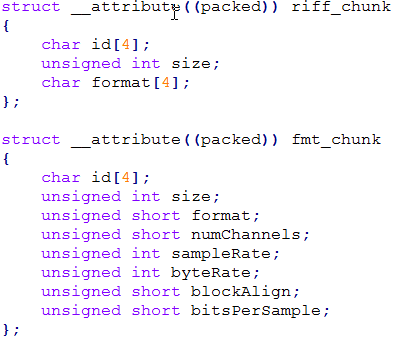
\includegraphics[width=7cm]{images/codesegment.png}
    \caption{Shows a sample data structure for extracting RIFF and fmt chunk of the WAV file.
 }
    \label{fig:code}
\end{figure}
\item \textbf{VeraCrypt}\\
\href{https://veracrypt.codeplex.com/wikipage?title=Downloads}{https://veracrypt.codeplex.com/wikipage?title=Downloads}\\
This freeware utility provides "on-the-fly encryption". This software is a fork of its predecessor TrueCrypt, which was discontinued by its development team due to security flaws. \cite{junestam2014open} This freeware utility is licensed under the Apache License 2.0 but due to previous licensing from TrueCrypt it is still subject to portions of the TrueCrypt License Version 3.0. Although the system built in this research can inject any file, we utilize the ability of this platform to quickly create an encrypted file system volume to be embedded. After the previously mentioned bash script, the VeraCrypt software requires additional information: a volume name, password, personal iterations multiplier (PIM) number, key file or a random sequence of 320 characters. 

One important feature of VeraCrypt worth mentioning is that much like its predecessor TrueCrypt, a deniable file system could be created within the encrypted file system volume. \cite{czeskis2008defeating} A deniable file system is essentially a hidden volume in the normal volume of an encrypted system. Since the encrypted system just has a fixed storage size, a smaller hidden volume could be nested within it. This hidden volume would be accessible through the VeraCrypt platform and would only be known to the user or intended recipient. They are considered deniable because unless you know the file system is present, there is absolutely no evidence that it itself exists. This particular method could be used in this security model to add another effective and advanced mechanism. This particular process could be performed k times nesting each volume and to a certain extent does not prove anything additional with regard to capacity. This does come with a space requirement for this because each system needs to be sufficiently larger than the payload contained within it. 

\end{itemize}

\subsection{Experiments}
Aside from the vast research needed to develop the experiment, the process of developing the StegoMax software platform with respect to editing the digital audio files came with three main phases: processing the data, determining the maximum effective capacity, and proving the steganographic effectiveness. 

The digital audio used in this experiment were a selection designed to draw conclusions from a variety of cases that would cover any edge concerns. These tests included audio files that were live, studio, loud, quiet, have periods of silence, periods of different pitches, several sounds, singular sounds, singing only, instrumental only, notes and tones only. Some specific songs selected are:\\
\\
Mark Ronson - Uptown Funk ft. Bruno Mars\\
Adele - Hello (Live at the NRJ Awards)\\
Taylor Swift - Shake It Off\\
Queen - Fat Bottom Girls\\
Redbone - Come And Get Your Love\\
Beethoven - Moonlight Sonata\\
\\
Processing the data initially required developing an understanding of the WAV file format and RIFF tagged file structure as previously mentioned. The platform resulted in developing simple structs to extract these sections for analysis as seen in Figure \ref{fig:code}. The next steps would involve accurately copying and editing file in a binary format. C++11 supports setting binary flags on the fstream to achieve this. After determining the data is extracted correctly, printing out the meta data sections and validate their results against proven software assured its accuracy. 

The determination of maximum effectiveness took some effort. Mathematically, the echo hiding and phase coding provide less theoretical capacity than spread spectrum and the least significant bit technique. Therefore, the first method considered was initially taking a spread spectrum approach. A smaller audio clip was used in exploring the data section by randomly changing the bits and bytes in a brute force manner to determine the success of modifying the digital audio file. This method was considerably ineffective, given the motivations of this research. 




The next steps were to explore the least significant approach and some other custom approaches. One custom approach was to utilize all the bits of a single channel to apply the payload. The WAV files used were stereo sound, meaning they had 2 channels of audio data, specifically left and right. The result can be seen in Figure \ref{fig:1channel}(a), which in hearing it, there was distinguishable loss of one signal and this approach was discarded. 

Lastly, a least significant bit approach was used. This was considerably effective and no noticeable audio difference could be discerned. In fact, no visual difference could be determined with the naked eye either using visualization tools. 



The next steps were to see if the next least significant bit made any difference. This process was repeated for all the least significant bits ranging from 1-bit to 8-bit in the 16-bit channel data sample. This part of the experiment showed considerable results. The 1-bit to 4-bit were completely hidden from signal, and there was no visible difference in the waveform visualization, as seen in Figure \ref{fig:1channel}(b). Once entering the 5-bit territory, on considerably higher volumes, a faint static was becoming apparently. From this point until 8 least significant 8-bits were used for the payload, the noise became more noticeable.

\href{https://www.youtube.com/watch?v=TLzsfvBW6Uo}{https://www.youtube.com/watch?v=TLzsfvBW6Uo} This is a video created to simply demonstrate the impact on audio quality ranging from 4-bit to 8-bit. This video has had several conversions from being converted into a WMV and being uploaded to YouTube, so the payload is destroyed, however the impact on the audio quality remains the same and the demonstration of increasing noise can be heard. This concluded the exploratory phase of determining the maximum capacity.

Lastly, proving the capacity with an embedding system and utilizing the high entropy system followed. A script was developed to resolve dependencies for VeraCrypt and assist in the creation of the encrypted FAT file system volume, however the StegoMax platform supports any payload that can fit in the particular WAV file being used. The determination if it will fit is using the 4-bit embedding approach. In the assumption section, the minimum capacity goal was used in the experimental phases. This required at minimum roughly 300 kilobytes worth of data capacity meaning the file size should be approximately four times larger being a 1.2 megabyte file. The desired results were achieved and successfully injected and extracted a payload of that size.

In the next sections, the results will be discussed in further detail along with the reverse engineering of the process with steganalysis.

\begin{figure}[tbh]
    \begin{subfigure}[t]{0.3\textwidth}
      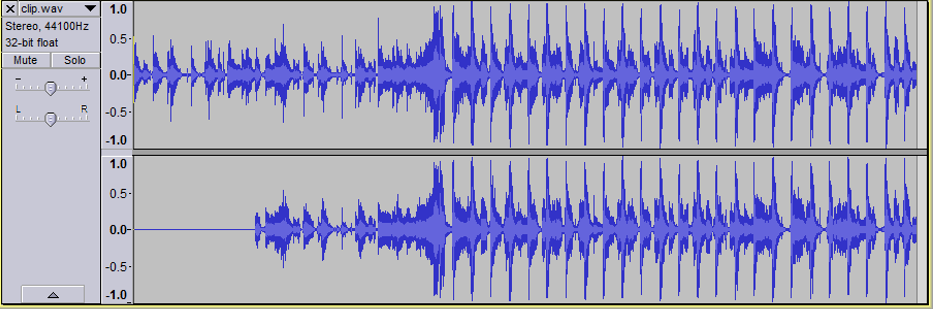
\includegraphics[width=8cm]{images/1channel.png}
      \caption{}
   \end{subfigure}
   \begin{subfigure}[t]{0.3\textwidth}
     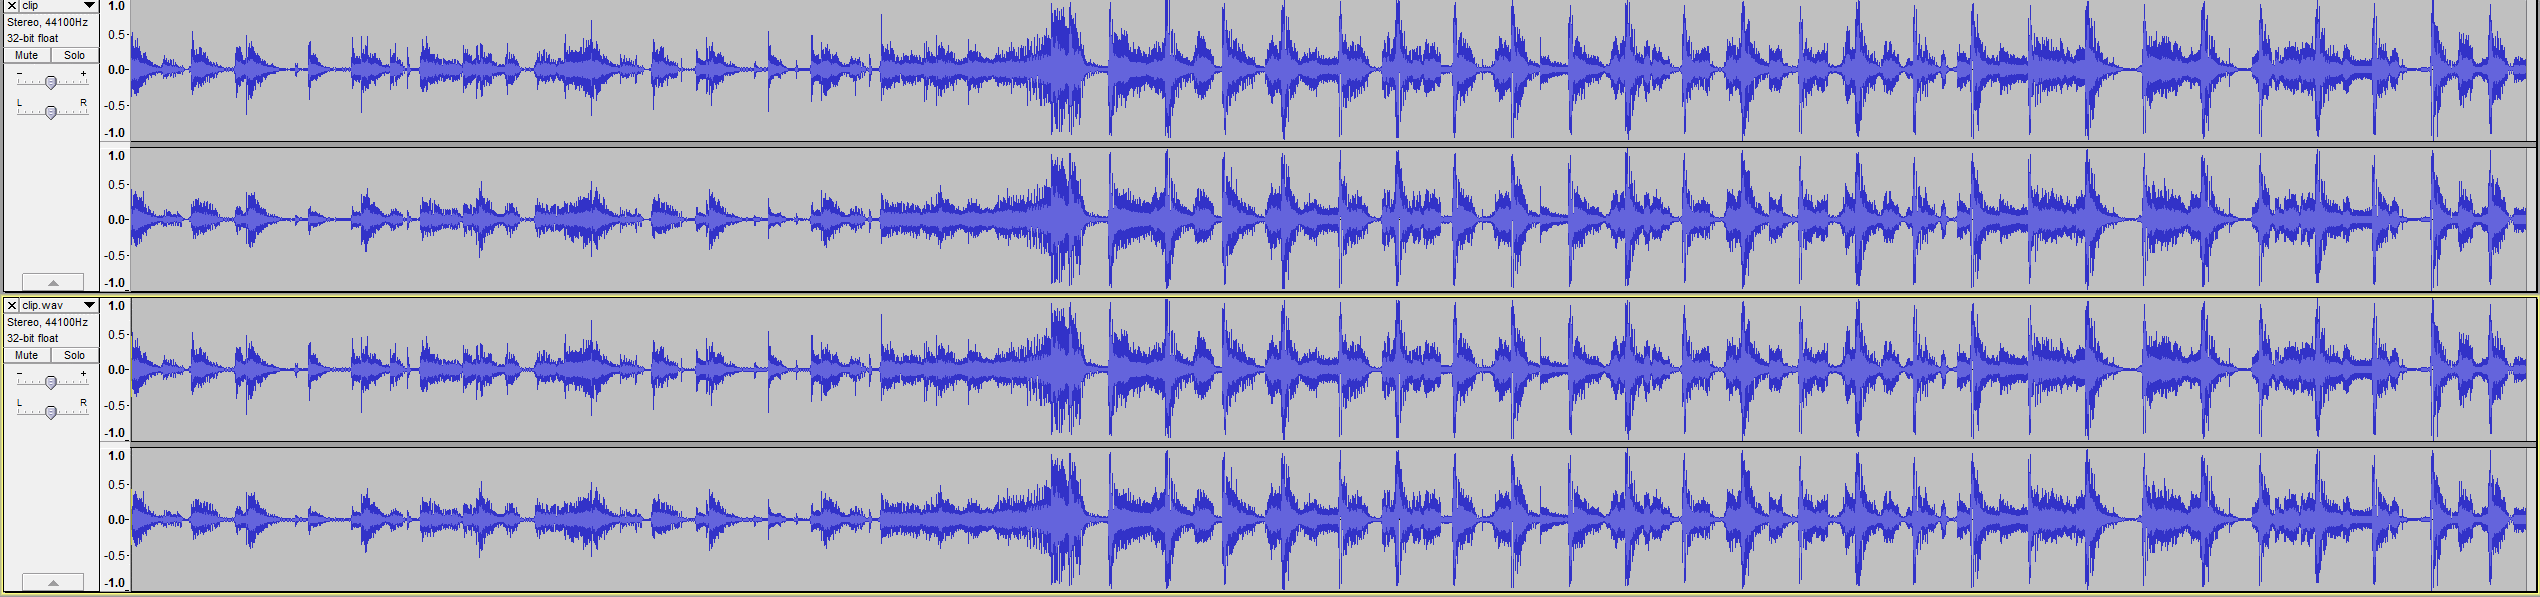
\includegraphics[width=8cm]{images/beforeafter.png}
     \caption{}
   \end{subfigure}
         \caption{This Audacity waveform visualization shows the first 300Kb of right channel samples being modified to support steganography. This method would raise suspicion and would be highly detectable. 
   }
    \label{fig:1channel}
\end{figure}

\begin{figure*}[ht]
    \centering
    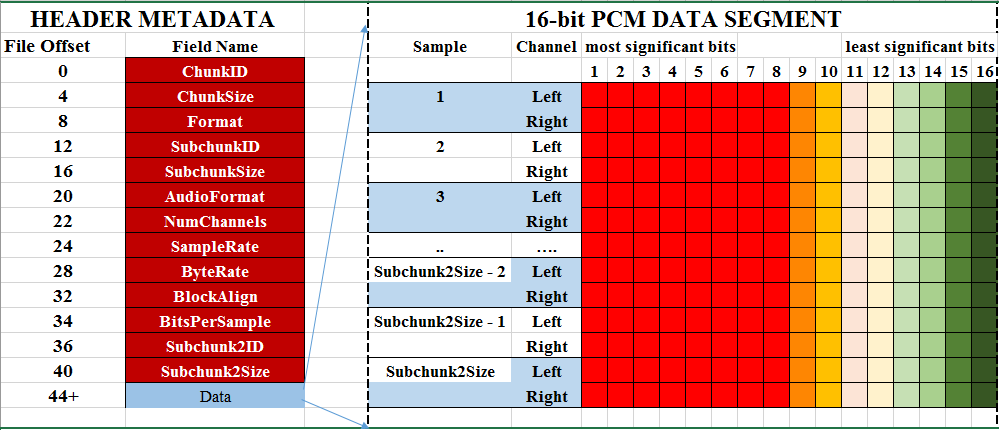
\includegraphics[width=13cm]{images/heat.png}
    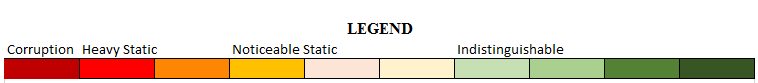
\includegraphics[width=13cm]{images/heatlegend.png}
    \caption{This shows a generalized theoretical bit usage for digital audio steganography in a 16-bit PCM WAV digital audio file. As seen from the legend, the darkest red indicates sections that cannot be modified without heavy risk of corruption. Although editing these sections will not always cause corruption, this heat map shows the general case. The rest of the data segment is ordered from most significant to least significant, showing the least significant 4 bits in green.
 }
    \label{fig:heatmap}
\end{figure*}

\section{VII. Experimental Results}
The measurement of success this research is determined by the ability for a passive adversary to determine that an alteration of significance exists. There are a few considerations that play into detecting the presence of hidden data, both previously mentioned assumptions and new concepts mentioned below. 

As previously discussed, the adversary is assumed to not have the original file, they will not be able to simply do a file hash on two files and determine they are different. That said, if the original file used to store the hidden data was a popular song, one might think to listen and compare with another recording of the song. 

There are several implications preventing this ability such as distortion or variance from other sources like YouTube. The YouTube video audio quality could be better or even worse, nonetheless being different in terms of sound. A live recording of a song could improve the stealthiness of the hidden data because there is already extra noise associated with the quality of recording.  

Another consideration is that file conversions, lossy compression, or other digital operations can happen at any point. In addition to that, there are different sources with different recordings such as live versus studio recordings. The live venues could be different times such as one recorded in New York and another in California. Even in the same venue, the recording could have been on different devices of varying quality at different areas of the venue. 

If the adversary is actively listening and expecting to hear something, they could possibly claim they detect a difference in some cases. They might believe something exists even if nothing is different. This statistical anomaly is described with testing the audio among individuals.

I surveyed nine people of varying backgrounds ranging from being knowledgeable of computer science and not. This was an oral survey involving questions about a single clip per person, using an embedded version and the original, and each case lasted less than five minutes each. I chose three clips that were used equally among them. The interactions were nearly identical with control questions. The survey interactions are described below:
\begin{quote}
"I am going to play a few songs for you and I will ask you a few questions about them." 
The first clip was played and this was always selected as the embedded version. The second clip is then played after that, except this is the original clip. "Are those the same two clips?" The answer was always yes. "My research is on data-hiding within audio files, I will now play you another clip with the data embedded." I then play again the original unedited file. The responses from this were mostly, "No, they all sound the same."   
\end{quote}
In two study cases, the individual claimed they could hear a difference between this final clip and the previous song, which were bit-identical files. However, in the event that they have 1000 files to sift through and there is one that may or may not contain a secret, they will be unlikely to determine it present in a reasonable amount of time. This survey was a brief extension into validating the claims made by the human auditory system section. 


Before settling on the clips provided in the scenario above, we satisfied our own threshold expectation on being able to detect suspicious noise. Figure \ref{fig:heatmap} shows a layout of the entire 16-bit PCM Microsoft WAV file without any optional meta data chunks. The coloring shows the noise or file corruption characteristic difference made when editing the files. The dark red primarily related to the format chunk cannot be used to provide space for generalized data. There may be tricks that can be applied to use them in a case by case situation, however, there are not bits that can be taken and used for every case. The data chunk shows a spectrum of what can be detected to what cannot be distinguished by sound alone. The legend and coloring provides for varying degrees of detection. After consuming the 4 least significant bits from each sample. \\rp


Effective Maximum Capacity = SUBCHUNK2SIZE * .25\\

Where SUBCHUNK2SIZE can be seen in Figure \ref{fig:heatmap} as included in the meta data. This cannot be calculated based on the total file size because of optional appendages that could exist. 


Lastly, as previously mentioned, these results are generalized among all songs based on the human auditory system and the bit relationship to the audio file. In specific settings where a certain type of audio file is used such as a live song recording, using 5 bit or 6 bit replacement might be completely acceptable because there is already a noise present.




\section{VIII. Steganalysis}
Steganalysis is the study of detecting hidden messages in steganography and can be considered the counterpart to cryptanalysis. The methods of steganalysis vary depending on the medium. In digital audio, different techniques and algorithms are used when detecting each method of steganography within a file. Spectrogram and wave analysis can be used to visual discern any unusual distortions within the audio file. 

Briefly discussing echo hiding and phase coding, since these methods were not used in this research, require statistical algorithmic approaches when attempting to discover steganography. "A statistical analysis of the phase difference in each audio segment can be used to monitor the change and train the classifiers to differentiate an embedded audio signal from a clean audio signal. The echo steganalysis algorithm statistically analyzes the peak frequency using short window extracting and then calculates the eighth high order center moments of peak frequency as feature vectors that are fed to a support vector machine, which is used as a classifier to differentiate between audio signals with and without data." \cite{meghanathan2010steganalysis}

Analyzing the distortions for this method is the most applicable method available. In the event that a spread spectrum technique was used, the distortions could potentially be seen by the naked eye in a waveform visualization or audio spectrogram. StegoMax cannot be seen from either as seen in Figure \ref{fig:1channel} (b) and Figure \ref{fig:spectrogram}. 

In steganography, it is commonly known that encrypted payloads such as that of StegoMax are incredibly complicated to distinguish from noise. Figure \ref{fig:spectrogram} shows how successful injecting the encrypted payload is with imitating the existing noise within the file, even if outside of audible hearing.

This figure shows the original file, containing artificially produced dead space in the first 0.05 seconds of the file. The resulting cover file after the payload has been embedded shows it is incredibly difficult to notice a difference and the resulting noise shown is inaudible, as previously mentioned. Remember, the adversary will not have the original file and this exact comparison would not be possible. Detection in this research model is impossible to the naked eye and indeterminate with computational operations.

\begin{figure*}[ht]
	\centering
    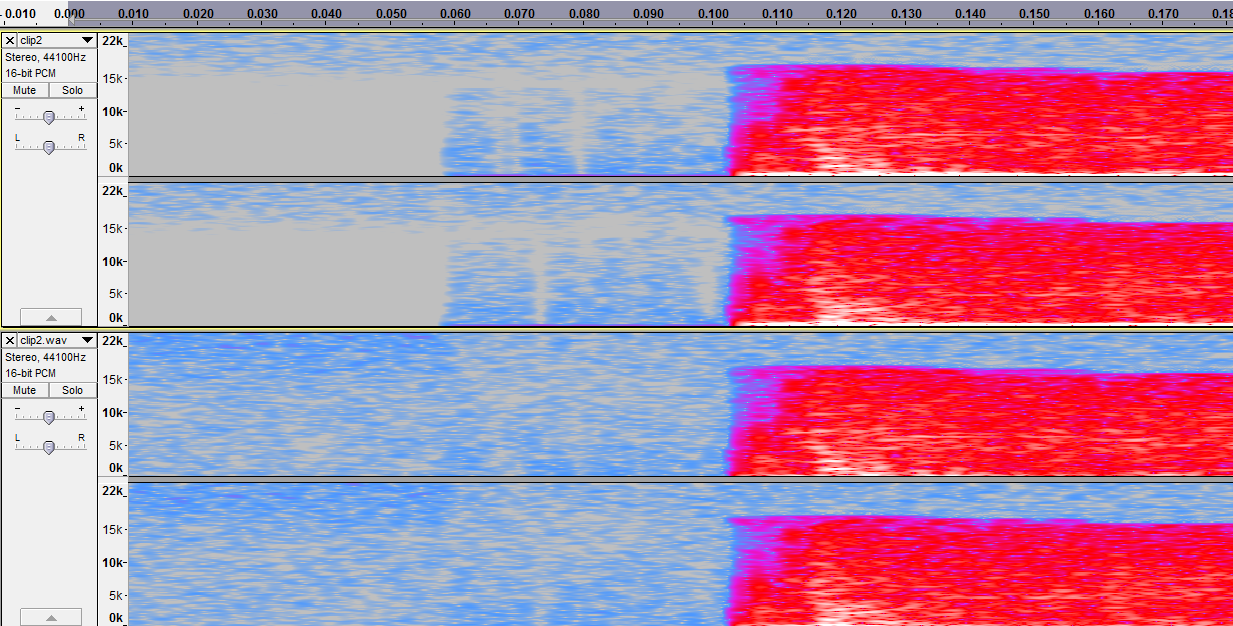
\includegraphics[width=15cm]{images/spectrogram.png}
	\caption{Spectrogram of an audio file sample with the original file on top and the modified file below. 
    }
    \label{fig:spectrogram}
\end{figure*}

Using machine learning and artificial intelligence methods have not been considered for this research. One method could be determining a relationship among the signal to noise ratio throughout the file and determine if there is any noise variances. This however would be immensely challenging and I cannot imagine successful. 

\section{IX. File Integrity}
In researching the maximum capacity of this audio file, we could extend this to other fields of research such as a relationship to the integrity of a file. Although this does not pertain to steganography directly, the research could provide insight on how research of integrity can be approached.

Using steganographic methods and determining the maximum capacity can also reveal the maximum values that can be damaged from normal operations such as from hard disk bit flipping. Bits in files occasionally can be flipped on hard disk over time due to the nature of magnetic disk. When this occurs, files could become damaged or corrupted.

An example could be said that there is approximately 75\% probability that the WAV digital audio file is unaffected from an incidental bit flip, assuming that each bit is equally probable to be flipped. Additionally, in Figure \ref{fig:heatmap}, if the first meta data chunks have any alterations, the WAV will likely be completely damaged.

\section{X. Conclusion}
The research has assessed the maximum capacity, the methods taken to achieve this effective upper bound, discussed the assumptions made to draw upon this conclusion and any considerations for this experiment. The effectiveness has been tested among surveyed individuals strengthening the human auditory system argument and the stegonagraphic system has successfully achieved the goals we set out to accomplish. Digital audio steganography as a means of data hiding has several positive and negative considerations. 

The positives involve the ability to conceal important data that might be imperative to national security or the lives of agents or members that are secretly communicating behind enemy lines. Utilizing digital audio steganography could provide them an open channel of secret communication that could evade detection. 

The negative is that digital audio steganography and applying techniques such as those mentioned in this research provide a strong means of hiding illicit activities for the "bad guys." Child pornography, illegal trades such as guns and drugs, and human trafficking can go about their business without arising suspicion from the authorities.

The measurement of maximum capacity for digital audio steganography in WAV files is approximately 25\% of the data chunk, specifically to the general case. As mentioned in the research in previous sections other cases storing a specific payload could result in greater yields such as the 5-bit or 6-bit approach using live performance audio, where environmental noise is already present in the media, could yield 31.5\% to 37.5\%. The choice to using more bits of the digital audio file would be determinate on the signal-to-noise requirements from the user and their need to conceal the information.

The resilience to detection through steganalysis has been assessed and shown first hand the spectrograms and the high entropy conclusions that can be made about the payload. This research applied the 256-bit AES encrypted FAT volume generated by the VeraCrypt software, which by Shannon Entropy is determined to have the maximum entropy by other supporting researches mentioned.



\section{XI. Future Work}
While our system can embed and extract files within a digital audio WAV files, future work consists of expansion into several other file types. In concurrent research of using WAV digital audio files, bitmap image file (BMP) files were explored as an image option for maximum capacity exploration. This research was not completed at the time of writing this document and no system functionality was designed to support this. In future implementations, we may add the ability for users to hide data within images and video. Additionally, we may choose to explore compressed options such as mp3 or mp4. 

In the preliminary stages of developing this system, we found that dealing with changing the bits in uncompressed formats is a sufficient starting place. The application of quantization tables and huffman coding would require more time in the research and is a reasonable domain for further exploration in later research. The huffman coding and quantization tables have algorithms in place in applications that parse them to read and determine the file's characteristics. We would have to rebuild these algorithms in some fashion in order to further understand the maximum capacity among compressed files. However, since the file is compressed, there is far less capacity available since changes made to these files are multiplicative.

Exploring the capacity and providing more research to the domain about the maximum capacities in video, images, and audio files can change the way steganography is used. Steganographic systems can become far more secure and robust given that they have plenty more storage space within a file to work with. Alternatively, file structures might be created to be resistant to steganography, crippling the ability to hide secret data within the file. 

Much like the DeepSound application mentioned in the related works, this application could be extended to multiple operating systems and support more file types.
\section{XII. Acknowledgments}
This paper was written for Andy Wang's Advanced Operating System class and the knowledge learned from this course has been monumental to growing and understanding more about pioneering research. I want to provide a special thanks to the individuals that contributed to the survey: Marian Bach, Alex Coyle, Adam Gorman, Jacob Harrelson, Daniel Hopson, Alexa Kyros, Garrett McLain, Andrew Rosenberg, and Sandy Stevenson. 

\bibliographystyle{iccc}
\bibliography{iccc}


\end{document}
